\section{Roll motion} \label{sec:roll}
The spring-mass-damper system, as shown in \autoref{fig:spring_mass_damper}, is a second-order linear ordinary differential equation (ODE) (\autoref{eq:spring_mass_damper}) that describes the motion of a mass attached to a spring and a damper. It is useful for understanding oscillatory and damping behavior.
\begin{figure}[h]
    \centering
    \includesvg[width=0.3\linewidth]{figures/Mass_spring_damper.svg}
    \caption{Mass-spring-damper model structure.}
    \label{fig:spring_mass_damper}
\end{figure}
\begin{equation} \label{eq:spring_mass_damper}
m\ddot{x} + c\dot{x} + kx = 0
\end{equation}

Roll motion without manoeuvres or external forces can be expressed by a nonlinear spring-mass-damper system \cite{himenoPredictionShipRoll1981},
\input{equations/roll_decay_equation_general_himeno}
\noindent where the subscript 44 indicates forces in the roll degree of freedom and the static stability of the ship is expressed as the stiffness $C_{44}(\phi)$ as a function of the roll angle $\phi$, the damping ($B_{44}(\dot{\phi})$) as a function of the roll velocity $\dot{\phi}$, and inertia $A_{44}$ connected to the roll acceleration $\ddot{\phi}$. The ship's roll motion can be observed under these conditions in a roll-decay test. The model is forced to an initial roll angle, as seen in \autoref{fig:rolldecay_initial}. It is then released (\autoref{fig:rolldecay_free}) and returns to equilibrium (\autoref{fig:rolldecay_equilibrium}). The model will pass the static water line as a result of its momentum and not stop until it has reached the end point on the other side (\autoref{fig:rolldecay_endpoint}). This motion starts a new cycle, with the model rolling back
once more. This new cycle results in oscillatory motion where potential energy is transferred to kinetic energy and back again to potential energy.
This oscillation would never end if it were not for the roll damping. Interactions between the ship and the water, such as friction, wave generation, eddy generation, and hydrodynamic lift, cause the ship to lose some of its energy. This energy loss causes the oscillation to decay over time, as seen in \autoref{fig:rolldecay}, which displays the time series for the roll angle.

\begin{figure}[H]
    \centering
    \begin{subfigure}[b,height=2cm]{0.22\textwidth}
         \centering
         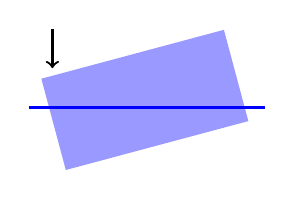
\begin{tikzpicture}

            \fill [blue!40, rotate around={15:(0,0.0)}] (-1.2,-0.5) rectangle (1.2,0.7);
            \draw[blue, thick] (-1.5,0) -- (1.5,0);
            \draw[black, thick, ->] (-1.2,1) -- (-1.2,0.5);
          
          \end{tikzpicture}
         \caption{The ship model is forces to an initial angle and then released}
         \label{fig:rolldecay_initial}
         \vspace{0.15cm}
     \end{subfigure}
     \hfill
     \begin{subfigure}[b,height=2cm]{0.22\textwidth}
         \centering
         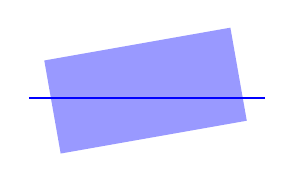
\begin{tikzpicture}

            \fill [blue!40, rotate around={10:(0,0.0)}] (-1.2,-0.5) rectangle (1.2,0.7);
            \draw[blue, thick] (-1.5,0) -- (1.5,0);
            
          \end{tikzpicture}
         \caption{Starts to roll back}
         \label{fig:rolldecay_free}
         \vspace{0.63cm}
     \end{subfigure}
     \hfill
     \begin{subfigure}[b,height=2cm]{0.22\textwidth}
         \centering
         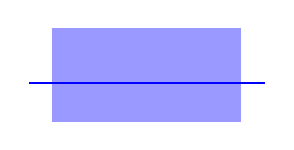
\begin{tikzpicture}

            \fill [blue!40, rotate around={0:(0,0.0)}] (-1.2,-0.5) rectangle (1.2,0.7);
            \draw[blue, thick] (-1.5,0) -- (1.5,0);
            
          \end{tikzpicture}
         \caption{Static water line.}
         \label{fig:rolldecay_equilibrium}
         \vspace{0.64cm}
     \end{subfigure}
    \hfill
     \begin{subfigure}[b,height=2cm]{0.22\textwidth}
         \centering
         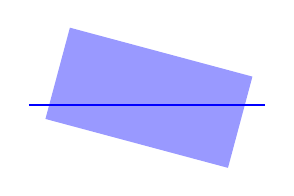
\begin{tikzpicture}

            \fill [blue!40, rotate around={-15:(0,0.0)}] (-1.2,-0.5) rectangle (1.2,0.7);
            \draw[blue, thick] (-1.5,0) -- (1.5,0);
            
          \end{tikzpicture}
         \caption{End point other side}
         \label{fig:rolldecay_endpoint}
         \vspace{0.36cm}
     \end{subfigure}
    \caption{Roll decay test.}
    \label{fig:rolldecay_procedure}
\end{figure}
\begin{figure}[H]
    \centering
    \includegraphics[width=0.7\linewidth]{kappa/images/rolldecay_example.pdf}
    \caption{Example roll decay signal.}
    \label{fig:rolldecay}
\end{figure}
The damping, $B_{44}\left(\dot{\phi}\right)$, can be expressed as an expansion series:  
\begin{equation}
    B_{44}\left(\dot{\phi}\right) = B_1\cdot\dot{\phi} + B_2\cdot\dot{\phi}\left|\dot{\phi}\right| + B_3\cdot\dot{\phi}^3 + ... + B_n\cdot\dot{\phi}^n
\end{equation}
 
\noindent This series can be truncated, allowing it to be expressed as a ``linear model'' (\autoref{eq:roll_decay_equation_himeno_linear}), \say{quadratic model} (\autoref{eq:roll_decay_equation_himeno_quadratic_b}), and ``cubic model'' (\autoref{eq:roll_decay_equation_cubic}). The stiffness function, $C_{44}(\phi)$, has been similarly expanded, only retaining the first term for the linear and quadratic models and the first three terms for the cubic model. 
\input{equations/roll_decay_equation_himeno_linear}
\input{equations/roll_decay_equation_himeno_quadratic_b}
\input{equations/roll_decay_equation_cubic}
%\subsection{Semi-empirical roll damping with Ikeda's method}
\label{sec:ikeda}
Ikeda's method \cite{ikeda_components_1978} divides roll damping into five damping components: the friction component $B_F$, the eddy component $B_E$, the lift component $B_L$, the wave component $B_W$, and the bilge keel component $B_{BK}$, as in the following Eq.(\ref{eq:ikeda}), 
\begin{equation} \label{eq:ikeda}
B_{44} = B_F + B_E + B_L + B_W + B_{BK}
\end{equation}
where the wave and eddy components require strip-theory based hydrodynamic analysis to obtain the ship's shape coefficients.